\documentclass[../../main.tex]{subfiles}


\subsection{Introducción a los microservicios}
\vspace{2mm}
\noindent
En primer lugar, vamos a intentar definir lo que es un microservicio. 
Aunque no hay una definición del todo clara, es interesante pens­ar en ellos 
como conjuntos auto contenidos que usualmente dan respuesta a pequeños problemas, 
normalmente mediante servicios, que se construyen alrededor de piezas claves para 
nuestro negocio. Estos microservicios deben ser procesos propios independientes 
capaces de comunicarse unos con otros con mecanismos ligeros, 
normalmente como recursos HTTP de una API. La mayoría de las veces se escriben 
en diferentes lenguajes de programación y no tienen por qué tener como base 
las mismas tecnologías de persistencia de datos.

Una arquitectura de microservicios se basa en la orquestación de los mismos
de manera adecuada. Esto nos da la ventaja de poder levantar réplicas de manera independiente, 
al contrario que en arquitecturas monolíticas, en las que toda la lógica de negocio 
se implementa en una solución única. En la Figura \ref{fig:monoliticsvsmicroservices} se pueden observar las diferencias entre las arquitecturas monolíticas y las arquitecturas de microservicios. El artículo de James Lewis y Martin Fowler 
\cite{martinfowler.com} que la incluye originalmente, resulta muy interesante para comprender el funcionamiento de los mismos.

\begin{figure}[H]
    \centering
    {%
    \setlength{\fboxsep}{0pt}%
    \setlength{\fboxrule}{1pt}%
    \fbox{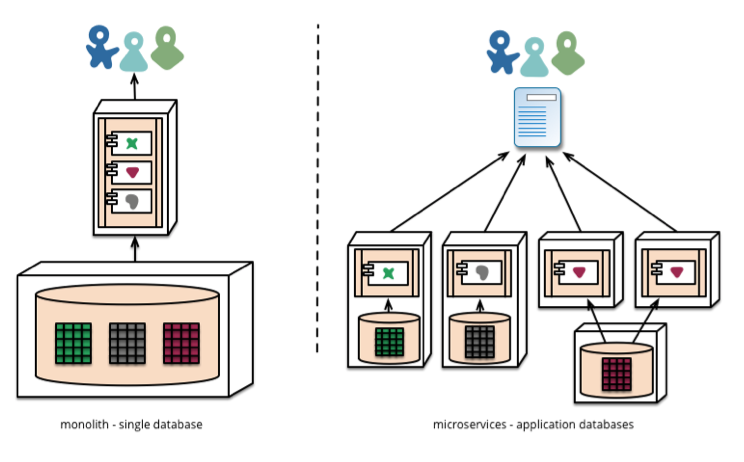
\includegraphics[width=0.55\textwidth]{monoliticsvsmicroservices}
    }%
    }%
    \caption{Arquitecturas monolíticas vs microservicios. \cite{martinfowler.com}}
    \label{fig:monoliticsvsmicroservices}
\end{figure}
\noindent
Para nuestra implementación contamos con la ayuda de contenedores de tipo \textit{Dockers}, y para orquestar los mismos utilizaremos 
la herramienta \textit{Docker-compose} que explicaremos detalladamente a continuación.

\subsection{Infraestructura como código(IaC)}
\vspace{2mm}
\noindent
Como hemos comentado anteriormente para orquestar estos microservicios utilizamos \textit{Docker}. 
Esto nos facilita mucho la vida a la hora de levantar réplicas de nuestros 
servicios de manera rápida, con el potencial añadido de incluso también poder llevar un control muy sencillo de las versiones
para los mismos, todo ello utilizando el concepto de infraestructura como código (IaC) \cite{morris_2016}.
\textit{Docker} es un software que proporciona contenedores, 
estos nos permiten tener una serie de recursos virtualizados que son completamente independientes entre sí, 
cada uno con características propias. Por ejemplo, espacios de nombres, 
sistema de archivos, etc. Todo ello hace que varios contenedores puedan funcionar 
en una sola instancia de Linux evitando así la sobrecarga de tener que iniciar
y mantener máquinas virtuales de manera independiente. Un sistema de \textit{Dockers} 
se basa en crear una capa que describe aquello que hay que hacer sobre las 
imágenes base de los contenedores en concreto. Sin meternos muy en profundidad 
en todas las opciones que \textit{Docker} nos ofrece, lo mejor para entender cómo se 
aprovisionan y se ejecutan contenedores mediante \textit{Docker} es ver un ejemplo:

\begin{lstlisting}
docker pull alpine
docker run -d --restart=always -p 80:80 alpine:version
\end{lstlisting}

En el código anterior, vemos cómo lo primero que debemos hacer es un \texttt{pull} de una 
imagen del repositorio oficial, que en nuestro caso es la que se ejecuta cuando 
ejecutamos el comando \texttt{docker run}. En el código anterior vemos cómo lo que hacemos 
es ejecutar un nuevo contenedor de esa imagen, a su vez, en nuestra máquina, 
cualquier petición que vaya al puerto 80 se redirigirá a ese contenedor también 
por el puerto 80. Otra de las opciones que vemos es que si hay una interrupción 
de nuestro contenedor, éste se reiniciará siempre gracias a la orden \texttt{restart=always}. La instrucción 
anterior es un ejemplo muy simple, dado que el cliente base de \textit{Docker} tiene muchas más 
órdenes que podemos aprender en la documentación oficial del mismo \cite{dockerdocumentation_2018}. Incluso, es posible
acceder a un nivel más interno de personalización de las máquinas que levantemos, siempre y cuando definamos el mismo de otra manera, en este caso con un 
\texttt{dockerfile}. cómo ejemplo de \texttt{dockerfile} (Listing \ref{lst:dockerfile}) veamos cómo a partir de la imagen de 
\textit{Neo4j}, utilizamos este archivo para personalizarla, instalando un complemento de datos 
espaciales en \textit{Neo4j} y las extensiones APOC.

\begin{lstlisting}[language=docker, caption={Ejemplo \texttt{dockerfile}.},captionpos=b, label={lst:dockerfile}]
FROM neo4j:3.1.4
MAINTAINER Manel Mena Vicente manel.mena@ual.es

ENV APOC_RELEASE 3.1.3.7
ENV APOC_RELEASES_URL https://github.com/neo4j-contrib/neo4j-apoc-procedures/releases/download
ENV APOC_PLUGIN_JAR apoc-${APOC_RELEASE}-all.jar
ENV APOC_PLUGIN_URL ${APOC_RELEASES_URL}/${APOC_RELEASE}/${APOC_PLUGIN_JAR}

RUN apk update \
    && apk add ca-certificates wget \
    && update-ca-certificates \
    && apk add openssl curl

RUN apk add --update zip unzip && rm -rf /var/cache/apk/*

RUN curl -s -L -o /var/lib/neo4j/plugins/neo4j-spatial-server-plugin.jar https://github.com/neo4j-contrib/spatial/files/1227950/neo4j-spatial-0.24-neo4j-3.1.4-server-plugin.zip

RUN curl --output /var/lib/neo4j/plugins/${APOC_PLUGIN_JAR} --location "${APOC_PLUGIN_URL}?raw=true"
\end{lstlisting}

En el archivo \texttt{dockerfile} podemos apreciar qué a partir de la imagen 
de \texttt{neo4j:3.1.4}, primero generamos una serie de variables de entorno, 
que después utilizamos para ejecutar órdenes básicas de Linux.

Junto con \textit{Docker}, es interesante utilizar una serie de herramientas que permiten 
aprovisionar contenedores de manera más sencilla, y así aprovechar todos los 
recursos de hardware de los que disponemos. Más concretamente \textit{Docker-compose}
y \textit{Docker-swarm}. Debido a los recursos disponibles a la hora de 
ejecutar nuestro proyecto (solo un equipo físico con recursos limitados), 
utilizar \textit{Docker-swarm} es bastante desmesurado, aun así es interesante conocer 
para que se utiliza el mismo. \textit{Docker-swarm} u otras herramientas similares como 
\textit{Kubernetes}, es interesante usarlas cuando contamos con bastantes recursos 
hardware, esto nos permite hacer un clúster de recursos donde todos ellos se agrupan 
para formar un único \textit{Docker engine}. A partir de la versión 1.12 de \textit{Docker}, 
el modo swarm ya está integrado en la herramienta base de \textit{Docker}.

El siguiente punto, y donde vamos a hacer un poco más de hincapié, es en ver y 
entender la herramienta \textit{Docker-compose}, la cual nos permite realizar la definición de la
configuración de nuestra infraestructura en un archivo YAML (\textbf{Y}et \textbf{A}nother \textbf{M}arkup \textbf{L}anguage) el cual configura los 
servicios de la aplicación y realiza todos procesos de creación y de arranque de 
los contenedores con un solo comando.

Primero veamos cómo es la organización de carpetas o scaffolding (Figura \ref{fig:scaffoldingWhayaBe}) de nuestra infraestructura.

\begin{figure}[H]
    \centering
    {%
    \setlength{\fboxsep}{0pt}%
    \setlength{\fboxrule}{1pt}%
    \fbox{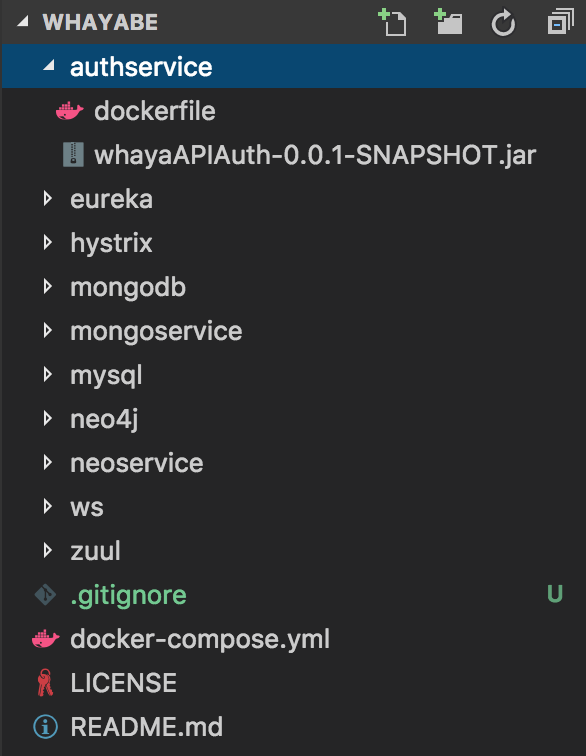
\includegraphics[width=0.4\textwidth]{scaffoldingWhayaBe.png}
    }%
    }%
    \caption{Scaffolding de WhayaBe.}
    \label{fig:scaffoldingWhayaBe}
\end{figure}
\noindent
Vemos que en la raíz contamos con el archivo \texttt{docker-compose.yml} 
en el que definimos toda la infraestructura. Aparte, los servicios que requieran 
configuración propia o lo que es lo mismo que no nazcan directamente de las 
imágenes base de \textit{Docker} sin configurar, también cuentan con un \texttt{dockerfile}
en el que se ejecutarán las órdenes de iniciación del contenedor en concreto.

Lo mejor para entender cómo funciona, es ver un pequeño fragmento del archivo \textit{Docker-compose} 
que orquesta nuestra infraestructura (Listing \ref{lst:dockercompose}).\\

\begin{lstlisting}[language=docker-compose,basicstyle=\ttfamily\small,caption={Ejemplo \texttt{docker-compose.yml}.},captionpos=b,label={lst:dockercompose}]
version: '3'
services:
  neo4j:
    container_name: neo4j
    build: neo4j
    restart: always
    ports:
     - 7474:7474
     - 7687:7687
     - 7473:7473
    environment:
     - NEO4J_AUTH=neo4j/secreto 
     - NEO4J_dbms_memory_heap_maxSize=2048M
     - NEO4J_dbms_memory_pagecache_size=2048M
    volumes:
     - ./neo4j/data:/data # provision the volumes
  mongo:
    container_name: mongodb 
    image: bitnami/mongodb:latest
    restart: always
    ports:
     - 27017:27017
    environment:
     - MONGODB_USERNAME=mongodb
     - MONGODB_PASSWORD=secreto
     - MONGODB_DATABASE=Whaya
    volumes:
     - ./mongodb/data:/bitnami
  neoservice:
    container_name: neoservice
    build: neoservice
    restart: always
    depends_on:
      - neo4j
      - zuul
      - eureka
      - rabbitmq
      - authservice
\end{lstlisting}

\noindent
Los tres servicios elegidos para mostrar cómo funciona \textit{docker-compose} son muy 
ilustrativos, dado que utilizan una serie de distintos tipos de configuración. 
En primer lugar, definimos la versión del cliente de \textit{docker-compose} que va a 
utilizar nuestro archivo de configuración. Para ello, utilizamos la palabra clave \texttt{version} a partir 
de ahí definimos cada uno de los servicios los cuales detallamos a continuación.

\begin{enumerate}[label=\alph*)]
    \item \textbf{Neo4j}: Primero asignamos un nombre con \texttt{container\_name}, la palabra clave \texttt{build} indica que para levantar este contenedor se debe utilizar el archivo \texttt{dockerfile} de la carpeta \textit{Neo4j}, \texttt{restart:always} nos permite indicar que queremos que si por alguna razón en el contenedor se produce un error insalvable o se cae por algún motivo este va a intentar siempre reiniciarse. En \texttt{ports} declaramos los puertos de escucha del contenedor; a posteriori con \texttt{environment} declaramos las variables de entorno que corresponden a ese contenedor y en \texttt{volumes} indicamos que se genere una copia 1 a 1 de una carpeta física de nuestra máquina a una carpeta virtual del contenedor, por lo que si se modifica algo en una carpeta de volumen, bien por la máquina virtual o por la física, esta se vea reflejada en la otra y viceversa. Gracias a ello podemos realizar una copia de la carpeta en otro dispositivo, y al levantar la infraestructura en ese otro dispositivo tengamos ya los datos que generó el contenedor anterior.
    \item \textbf{MongoDb}: Este servicio se diferencia del anterior tan solo en que no parte de la palabra clave \texttt{build}, si no que nace desde la imagen original de \textit{MongoDb} proporcionada por la compañía \textit{Bitnami} a partir del comando \texttt{image}. En ella no realizamos ninguna personalización mas allá de modificar los valores por defecto de algunas variables de entorno de la misma.
    \item \textbf{Neoservice}: Ésta vuelve a ser como la primera imagen, pero vemos como se aprecia un nuevo comando, mas concretamente \texttt{depends\_on} el cual nos proporciona la posibilidad de iniciar el contenedor en concreto después de lo contenedores que están bajo \texttt{depends\_on}.
\end{enumerate}
\noindent
Es interesante fijarnos en que \textit{Docker} nos permite levantar todo tipo de servicios virtuales, no solo
servidores web, si no también bases de datos, o casi cualquier otra cosa que se nos ocurra. De hecho,
el mundo en general de la virtualización está virando hacia el ecosistema \textit{Docker} de manera fulgurante.
Compañías como Microsoft con su nube Azure, Google con ComputeEngine y CloudSoftware con OpenStack, ya 
ofrecen la posibilidad de utilizar archivos de configuración \textit{Docker} para levantar de 
manera rápida servicios en sus Clouds.

A continuación vamos a nombrar cada uno de los contenedores gestionados con \textit{Docker} en nuestra arquitectura, así como
una breve descripción de la función cada uno de ellos:

\begin{itemize}
\item \textbf{Neo4j}: Base de datos que guarda los usuarios junto con relaciones entre los mismos y los encuentros
organizados.
\item \textbf{Neo4jService}: Servicio que gestiona los datos relacionados con los usuarios y encuentros organizados por los mismos.
\item \textbf{MongoDb}: \texttt{Data Lake} en el que se guardan de manera anónima toda la información
de las posiciones de los usuarios mes a mes.  
\item \textbf{MongoService}: Servicio que gestiona el histórico de datos de geoposicionamiento de nuestro sistema. 
\item \textbf{MySql}: Base de datos donde guardamos todo lo referente a la autorización y autenticación de los 
usuarios en nuestro sistema respetando la definición de seguridad OAuth 2.0.
\item \textbf{AuthService}: Servicio que recibe las peticiones de nuestro sistema OAuth 2.0.
\item \textbf{Ws}: Servicio de Socket.io que se encarga de manejar todos los datos en tiempo real de nuestra aplicación.
\item \textbf{Eureka}: Componente de Netflix OSS que actúa de registro de servicios. 
\item \textbf{Zuul}: Componente de Netflix OSS que proporciona una puerta de enlace para acceder al resto de servicios.
\item \textbf{Hystrix}: Componente de Netflix OSS que controla el estado de las peticiones de nuestro sistema que nos
ayuda a implementar el patrón \textit{Circuit Breaker} en el mismo. Este patrón lo explicaremos posteriormente.
\item \textbf{Rabbitmq}: Sistema de gestión de cola de mensajes que permite la comunicación entre los componentes de
nuestra arquitectura. Dando soporte a \textit{Hystrix}, componente esencial para la detección de errores en la comunicación en arquitecturas compatibles con Netflix OSS. 
\end{itemize}
\noindent
La mayoría de estos servicios serán explicados con más detalle posteriormente. Esto tan solo es una primera aproximación para que tengamos
una idea de los contenedores que gestionamos mediante la herramienta \textit{Docker}.

\subsection{Arquitectura de microservicios}
\vspace{2mm}
\noindent
Una buena práctica es comenzar partiendo de un pequeño esquema sobre cómo vamos a partir nuestros 
microservicios. Esto lo hacemos para delimitar el tipo de servicios que utilizamos en nuestra
arquitectura. Para ello, nuestro subsistema de \textit{back-end} contará en un primer momento con 2 niveles básicos o capas 
que se detallan a continuación:
\begin{itemize}
\item \textbf{DB Services}. Estos servicios son básicamente aquellos que levantan las bases de datos
que controlan la persistencia de los datos manejados en nuestra lógica de negocio.
\item \textbf{API Services}. Estos servicios son los que controlan por un lado nuestra lógica de negocio
y por otro exponen la funcionalidad de manera externa, permitiendo a aplicaciones de terceros hacer uso
de los mismos (siempre y cuando sean \textit{trusted apps}).
\end{itemize}
\noindent
Dentro de estos dos primeros niveles básicos, contamos con los que son replicables a nivel de infraestructura,
véase los servicios incluidos en la capa de API Services, y los que no, aquellos 
que pertenecen a la capa de DB Services. En esta última tenemos la persistencia de datos,
y replicarlos a nivel de infraestructura podría dar lugar a inconsistencia en los mismos.
Por tanto, si se desea hace una réplica de estos servicios se debe hacer a nivel 
de base de datos. Esto hace que nuestra arquitectura básica objetivo sea la representada 
en la Figura \ref{fig:ArquitecturaObjetivo}.
\begin{figure}[H]
\centering
{%
\setlength{\fboxsep}{0pt}%
\setlength{\fboxrule}{1pt}%
\fbox{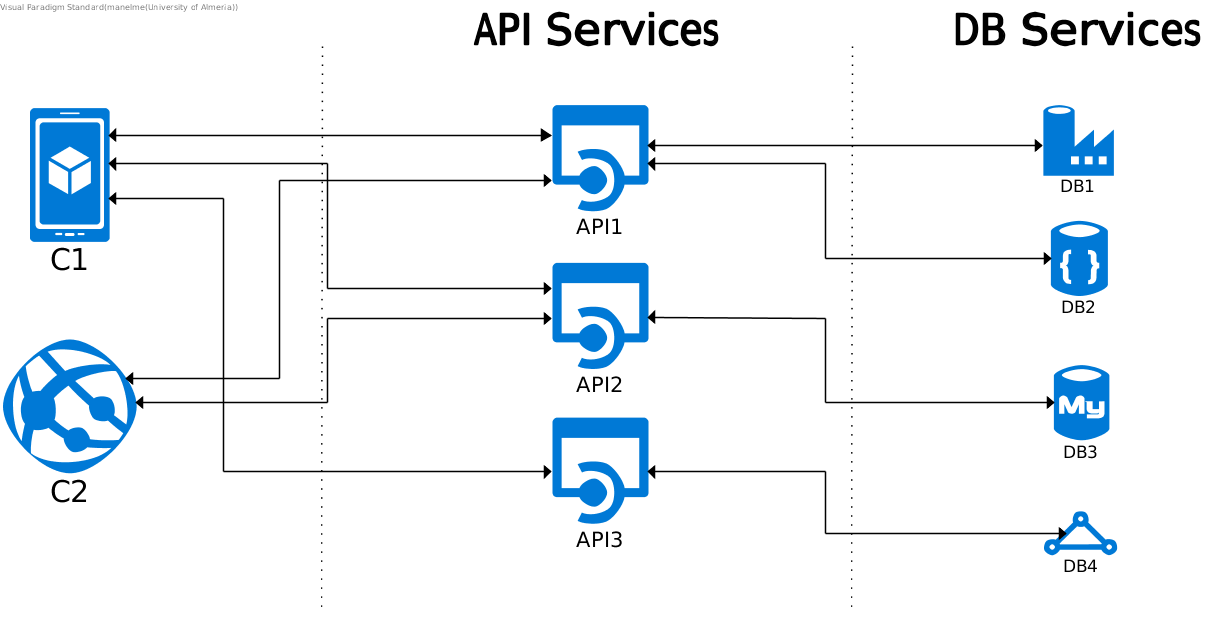
\includegraphics[width=0.6\textwidth]{ArquitecturaObjetivo}}%
}%
\caption{Arquitetura básica objetivo Whaya.}
\label{fig:ArquitecturaObjetivo}
\end{figure}
\noindent
A parte de lo que seria la arquitectura básica de nuestros microservicios, contamos con un nivel más
que denominamos como ``capa de orquestación de microservicios", la cual será explicada mas adelante.

El hecho de desplegar la arquitectura mediante microservicios conlleva una serie de problemas que es conveniente plantearse
incluso antes de desarrollar nuestro sistema, como por ejemplo:

\begin{itemize}
\item \textbf{Número de microservicios que desplegamos}. Cada microservicio tiene su propia configuración y ocupa sus puertos,
lo cual aumenta la complejidad de nuestro sistema en general y esto se puede convertir en un problema de envergadura a la hora
de mantener el sistema si lo hacemos de manera manual, por lo que tenemos que intentar alcanzar un compromiso entre la separación de 
microservicios y la granularidad que le vamos a dar a los mismos.
\item \textbf{Seguimiento de estado de los microservicios}. Otra problemática es que cuando tenemos un sistema
con tantas pieza pequeñas es difícil realizar un seguimiento de cada una de ellas y comprobar que todas están listas
para ser utilizadas y no hay ningún problema. Este problema se da en menor medida cuando contamos con una arquitectura monolítica.
\item \textbf{Mantener el seguimiento de la información y evitar fallos en cadena}. Dado que intrínsecamente los microservicios pueden
y deben comunicarse entre sí, es interesante intentar llevar un seguimiento del flujo y estado de la información. Dado que si no
tenemos cuidado con este punto se puede dar el caso de que, o bien el tiempo de respuesta de nuestros microservicios se vea muy mermado
si la información pasa por muchos microservicios, o bien se produzca un fallo en uno de ellos y genere una reacción en cadena.
\item \textbf{Asegurarnos que solo ciertos servicios estan expuestos al exterior}. Es necesario que solo ciertos servicios sean
expuestos al exterior. En nuestro caso los únicos visibles serán los servicios de tipo API Services, aunque como explicaremos posteriormente,
solo tendremos un servicio expuesto a puerto publico (\textit{Zuul}, un servicio de la capa de orquestación).
\item \textbf{Cómo proveer de seguridad nuestros servicios API}. Al contar con más de un microservicio en nuestro sistema, tenemos que plantearnos
cómo anteponer la seguridad desde otra perpectiva distinta a como lo haríamos en un servicio monolítico. En nuestro caso contamos con dos alternativas
que serán comentadas a la hora de explicar la orquestación de la arquitectura. 
\end{itemize}
\noindent
Para dar solución a estos problemas contamos con una nueva capa en nuestra arquitectura, la que hemos denominado la \textbf{capa de orquestación}.\\

\subsection{Orquestación de microservicios/patrones de sistemas}
\vspace{2mm}
\noindent
En esta capa vamos a levantar una serie de microservicios que nos ayuden a gestionar, monitorizar y exponer de forma segura el resto de microservicios así
como la comunicación entre los mismos. Para ello contamos con la ayuda de un framework de componentes altamente probados \textbf{Netflix OSS}. Nuestra solución
de orquestación se basa en los siguientes componentes:

\begin{enumerate}[label=\alph*)]
\item \textbf{Servicio de descubrimiento}. \textit{Eureka} es un microservicio que levantamos para ayudarnos a llevar un seguimiento de los microservicios.
Cuando levantamos los mismos, estos hacen una llamada a ese servicio de descrubrimiento para decirle quienes son y en qué estado están. A su vez, un microservicio podrá preguntar
por otro siempre y cuando ambos estén registrados en \textit{Eureka}, gracias a una API de descubrimiento de servicios que se incluye en el mismo.
\item \textbf{Circuit Breaker}. \textit{Hystrix} es otro microservicio de nuestra capa de orquestación que nos ayuda a implementar el patrón \textit{Circuit Breaker}.
Este patrón se utiliza para evitar posibles errores en cadena, para entenderlo de mejor manera es recomendable leer la entrada al blog de Martin Fowler, \textit{Circuit Breaker} \cite{CircuitBreaker}. 
Pero por tener una idea básica, \textit{Hystrix} se encarga de ver todas las peticiones y sus respuestas en nuestra arquitectura. Si alguna de estas peticiones muestra de manera continua errores, \textit{Hystrix} se encargará
de lanzar una respuesta predefinida en puesto de sobrecargar nuestro servicio con peticiones que van a ser erroneas, basicamente se abre el circuito. No obstante, cada cierto periodo de tiempo \textit{Hystrix} se
va a encargar de comprobar ese método del servicio en concreto que tiene abierto el circuito, a ver si vuelve a funcionar correctamente, momento en el que cerrará el circuito. En la Figura \ref{fig:CircuitBreaker} se ilustra esto mediante un diagrama de secuencias.

\begin{figure}[H]
\centering
{%
\setlength{\fboxsep}{0pt}%
\setlength{\fboxrule}{1pt}%
\fbox{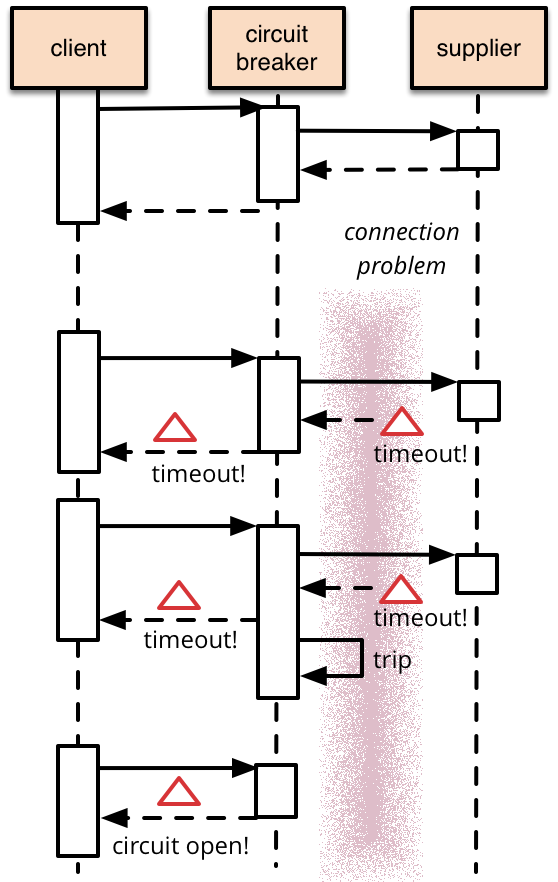
\includegraphics[width=0.4\textwidth]{circuitBreaker}}%
}%
\caption{Patrón \textit{Circuit Breaker}. \cite{CircuitBreaker}}
\label{fig:CircuitBreaker}
\end{figure}

\item \textbf{Monitorización}. Gracias a que tenemos esos \textit{circuits breakers} podemos llevar una monitorización al detalle de cada uno de los recursos expuestos en nuestros microservicios. Para ello utilizamos \textit{Turbine}, que se encarga de monitorizar
todos los métodos de nuestros microservicios que tengan la posibilidad de cortocircuitarse. 
\item \textbf{Edge Service}. \textit{Zuul} es otro microservicio proveniente del framework de Netflix OSS que nos ayuda a implementar el patrón de sistemas puerta de enlace. A través del mismo expondremos al exterior
el resto de servicios para prevenir acceso no autorizado a los recursos, el mismo utilizará de base, sistemas de balanceo de carga (con ayuda de Ribbon) y enrutamiento dinámico dentro de nuestra arquitectura. Dado que como
comentamos anteriormente podremos tener réplicas de los servicios API dentro de nuestro sistema, todo registrado en nuestro sistema de descubrimiento. \textit{Zuul} actuará como un servidor dinámico de proxy reverso,
el cual no será necesario actualizar manualmente cuando un nuevo servicio se añada a nuestra arquitectura.
\item \textbf{OAuth 2.0}. \texttt{AuthService} es un microservicio que está entre la capa de orquestación y la capa de servicios API. Dado que si bien es un servicio que ofrece
una serie de recursos al exterior, en mayor medida lo usaremos en cada uno de los servicios internos API para comprobar si el usuario esta autenticado y autorizado para acceder a un recurso en concreto. Mas adelande explicaremos
detalladamente este microservicio así como el protocolo de seguridad que implementa. 
\end{enumerate}
\noindent
Una vez hemos enumerado cada uno de los servicios de la capa de orquestación de nuestra arquitectura, vamos a ilustrarlo en la Figura \ref{fig:ArquitecturaObjetivoFinal}.
\begin{figure}[H]
\centering
{%
\setlength{\fboxsep}{0pt}%
\setlength{\fboxrule}{1pt}%
\fbox{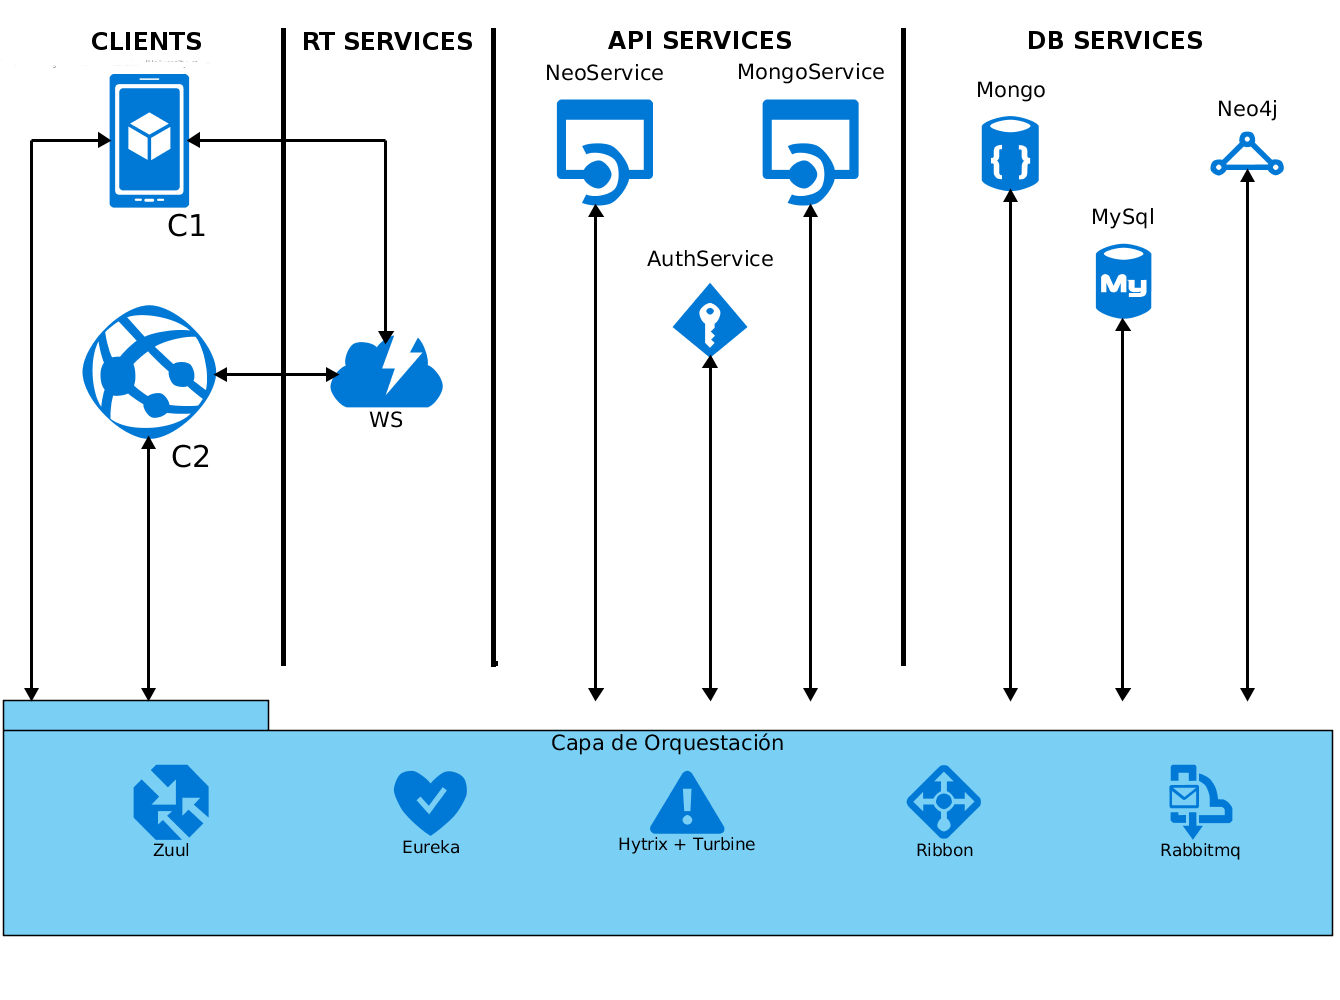
\includegraphics[width=0.72\textwidth]{ArquitecturaObjetivoFinal}}%
}%
\caption{Arquitetura final de Whaya.}
\label{fig:ArquitecturaObjetivoFinal}
\end{figure}

Esta figura pretende mostrar que los clientes deben de utilizar la capa de orquestación para comunicarse con los servicios API, y estos a su vez deberán comunicarse con los servicios DB también mediante la capa de orquestación. Todos ellos tomando como punto de confluencia de comunicación a \textit{Zuul}. Éste, gracias a el resto de servicios de
orquestación, será capaz de determinar las rutas y el estado de todos ellos. En el caso de los servicios API, de manera dinámica, y en el caso de los servicios DB con rutas ya preestablecidas.

El caso del servicio de datos en tiempo real es un tanto especial, ya que es el único que no utiliza nuestra capa de orquestación. A modo resumen pasamos a enumerar características comunes a los servicios de cada capa.
\begin{enumerate}[label=\alph*)]
    \item Servicios API. En esta capa contamos con los microservicios que responden a las peticiones de los clientes, entre sus características contamos con que todos ellos procederán a registrarse en \textit{Eureka} cuando sean levantados; \textit{Zuul} genera de manera dinámica rutas para su comunicación con otros elementos; la replicación de los mismos se puede realizar a nivel de infraestructura por lo que gracias a \textit{Ribbon}, \textit{Zuul} podrá de manera dinámica levantar réplicas si lo considera oportuno para aliviar el nivel de carga de los mismos.
    \item Servicios DB. Esta capa cuenta con lo servicios relacionados con la persistencia de datos, como características principales la replicación de los mismos se realiza a nivel de base de datos, dado que de lo contrario podría producirse inconsistencia en los datos. Al contrario que los servicios de API estos deben establecer rutas predefinidas en \textit{Zuul} dado que en primera instancia no están preparados para registrarse por sí solos en \textit{Eureka}, por lo que \textit{Zuul} no tiene visibilidad de manera automática al estado de los mismos.
    \item Servicio RealTime. No cuenta con nigún tipo de replicación, al contrario que los servicios de las otras dos capas. Comparte con los servicios DB el hecho de que no se registra en \textit{Eureka}, pero a su vez cuenta con una salvedad, al contrario que estos la comunicación de este servicio utiliza el protocolo \textit{WebSocket}, esto conlleva que no se lleve bien con \textit{Zuul}. Las características de este servicio provocan que por lo pronto se quede fuera de la capa de orquestación.
    \item Servicios Orquestación. Todos los servicios de esta capa, excepto \textit{Zuul}, tienen la capacidad de replicarse a nivel de infraestructura, a su vez todos ellos son los que se encargan de controlar la comunicación entre el resto de capas estableciendo control en el flujo de información.
\end{enumerate}
\subsection{Seguridad de microservicios}
\vspace{2mm}
\noindent
Para proteger la seguridad de nuestra arquitectura de microservicios contamos principalmente con dos técnicas complementarias. 
\subsubsection{Comunicación segura HTTPs}
\vspace{2mm}
\noindent
En primer lugar conviene recordar que nuestra arquitectura solo tiene un punto de acceso, más concretamente \textit{Zuul}, esto nos ayuda
a que simplemente en ese punto tengamos levantado todo lo relacionado con \texttt{https} de nuestros servicios, ya que solo aquí tendremos comunicaciones con sistemas externos. Por lo tanto, no hay necesidad de tener que implementar, en la red
interna generada por \textit{Docker}, comunicación mediante protocolos seguros, ya que tan solo en esa red tendremos visibilidad a los datos manejados en los microservicios.

Para poder firmar la seguridad del protocolo \texttt{https} hemos utilizado la herramienta proporcionada por la \textbf{Linux Foundation} \texttt{Let's Encrypt}
\cite{letsencrypt}. Ya que aunque siempre tenemos la opción de generar un certificado nosotros mismos, y dado que no somos una agencia certificadora de confianza en ningún navegador, estos nos detectarían como una página no segura,
imposibilitando el acceso a nuestro \textit{back-end}. Gracias a \texttt{let's encrypt} podemos firmar de forma segura y con confianza nuestro protocolo de seguridad, y como hemos comentado antes, tan solo debemos de hacerlo
en un punto, \textit{Zuul}.

Por otro lado, para controlar tanto la autentificación como la autorización de nuestros microservicios, hemos realizado la implementación del protocolo OAuth 2.0 \cite{oauth}. Para ello, implementamos un servidor OAuth (como microservicio), y distintos clientes en cada
uno de los microservicios que hacen uso de este servidor de OAuth para verificar que el usuario tiene acceso a los recursos a los que realiza la petición. La ventaja de utilizar este tipo de protocolo de serguridad es que contamos con la posibilidad de que nuestros microservicios 
realicen la comprobación de credenciales, no solo con nuestro servidor, sino también con otros servidores de confianza como pueden ser Google, Facebook, LinkedIn, etc. Ya que estos ofrecen la posibilidad mediante API de actuar como servidores de autenticación con las cuentas de sus usuarios.

Para comprender este protocolo y entender cómo implementarlo ,existen gran variedad de recursos entre los que se incluye \textit{OAuth 2.0 Cookbook: Protect your web applications using Spring Security} \cite{nascimento2017oauth}. No obstante en el siguiente punto vamos a intentar explicar de manera sencilla
cómo funciona este protocolo.

\subsubsection{OAuth 2.0}
\vspace{2mm}
\noindent
OAuth 2 es la segunda versión del protocolo o framework de OAuth. Este protocolo permite acceso limitado a recursos
de servicios HTTP, bien a través del ``Resource Owner'' o bien permitiendo el acceso a recurso de terceros para que estos puedan acceder a la misma
todo a través de un cliente autorizado.

El protocolo cuenta con cuatro figuras básicas, a saber:
\begin{enumerate}[label=\alph*)]
\item \textbf{Resource Owner}: Normalmente nosotros.
\item \textbf{Resource Server}: Éste viene a ser el servidor que aloja los datos que estan protegido por el protocolo.
\item \textbf{Cliente}: La aplicacion que pide el acceso a el \texttt{Resource Server}. Basicamente lo que viene a ser nuestra aplicación web, movil, etc.
\item \textbf{Authorization Server}: El server que proporciona el token de acceso al \texttt{cliente}. Este token será utilizado por el cliente para acceder
al \texttt{Resource Server}. En algunos casos \texttt{Authorization Server} esta embebido en el mismo \texttt{Resource Server}, no siendo nuestro caso ya que nuestro
servidor de autorización es un microservicio a parte.    
\end{enumerate}
\noindent
Lo siguiente es hablar de qué es un token, y de qué tipos de tokens contamos en OAuth 2. Los tokens vienen a ser cadenas de texto aleatorias generadas por \texttt{Authorization Server}, las cuales los clientes
deben pasar en las peticiones a los \texttt{Resource Servers}. Contamos con dos tipos:

\begin{enumerate}[label=\alph*)]
\item \textbf{Access Token}: Permite que los datos de usuarios se accedan desde una aplicacion de terceros. Este token es mandado por el cliente bien como un parámetro,
o bien como un componente de la cabecera de una petición hacia el \texttt{Resource Server}. Es importante comentar que estos tokens en el protocolo OAuth 2 tienen un tiempo
de vida limitado que el \texttt{Authorization Server} define. Tiene que ser lo más confidencial posible pero muchas veces esto se convierte en algo muy difícil de asegurar,
ya que en la mayoría de los casos los clientes tienden a ser aplicaciones web o derivados, que para no estar pidiendo la autorización de usuarios continuamente, guardan los token en \texttt{session}.
\item \textbf{Refresh Token}: Este token al contrario que el anterior, tiene que ir de la mano de un \texttt{Access Token}, y se utiliza solo en el caso de que este último haya expirado. Cuando se realize esta petición
de refresco de token, nuestro \texttt{Authorization Server} comunicará al cliente un nuevo par de \texttt{Access Token - Refresh Token}.
\end{enumerate}
\noindent
En el protocolo contamos con varias capas de autorización. La primera de ellas es la llamada \texttt{scope}, que es un parámetro que va asociado con los tokens generados que permiten limitar los derechos de acceso a nuetros recursos a nivel token.
El servidor de autorización es el que limita los \texttt{scopes} generados. El cliente debe de mandar el \texttt{scope} que quiere utilizar cuando realiza una petición.

Otra capa de autorización sería el registro como cliente de nuestra aplicación. Nuestro servicio de autorización no cuenta tan solo con la autentificación de usuarios, sino que también debe ser autorizada la aplicación que esta usando el mismo.
Esto confirma que se puede dar el caso de que un usuario esté registrado en el sistema, pero que al intentar entrar con un cliente no autorizado, no se le permita el acceso a recursos. El registro de clientes (aplicaciones) cuenta con cuatro parametros
principales a la hora de realizarse:

\begin{enumerate}[label=\alph*)]
\item \textbf{Application Name}: Básicamente el nombre por el que identificaremos la aplicación.
\item \textbf{Grant Type(s)}: Tipos de autorización que serán usadas por el cliente.
\item \textbf{Redirect URLs}: URLs del cliente que este utilizará a la hora de recibir códigos de autorización.
\item \textbf{Javascript Origin(opcional)}: El nombre del host al cual le será permitido pedir datos al \texttt{Resource Server} mediante XMLHttpRequest.
\end{enumerate}
\noindent
Una vez se haga el registro del cliente, a éste se le asociará un \texttt{Client Id}, que viene a ser una cadena de texto única y un \texttt{Client Secret} una clave secreta para identificar a ese cliente que se ha de guardar en sitio seguro.
Estos dos parametros tendrán que ser enviados con cada petición que se realize de recuperación o consulta de tokens.

Anteriormente hablamos de los tipos de autorización, en el caso del protocolo OAuth 2 existen cuatro tipos basicos de tipos de autorización, de los cuales presentaremos una pequeña explicación de cuando se usan y un diagrama de secuencia que ilustre un escenario de uso de cada uno de los mismos:

\begin{enumerate}[label=\alph*)]
\item \textbf{Authorization Code Grant} (Figura \ref{fig:AuthorizationCodeGrantFlow}). Este tipo debería ser utilizado cuando el cliente sea un web server. Ya que nos permite acceso a un token que puede ser renovado continuamente con el refresh token siempre y cuando este lo permita.
Normalmente el token de acceso se guarda como una variable de \texttt{session} en nuestro navegador y el cliente nunca tiene porqué verlo.

\begin{figure}[H]
\centering
{%
\setlength{\fboxsep}{0pt}%
\setlength{\fboxrule}{1pt}%
\fbox{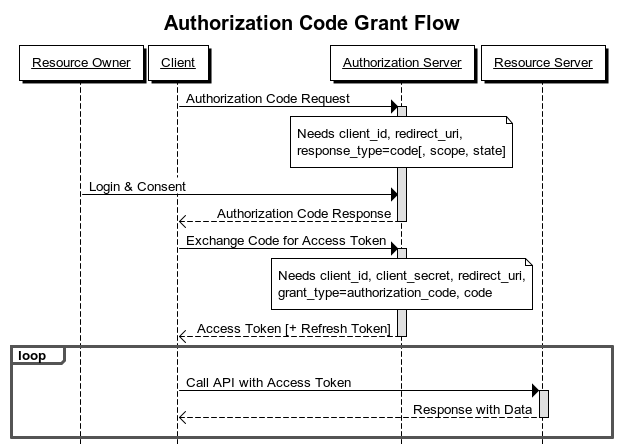
\includegraphics[width=0.7\textwidth]{AuthorizationCodeGF}}%
}%
\caption{Authorization Code Grant Flow.}
\label{fig:AuthorizationCodeGrantFlow}
\end{figure}

\item \textbf{Implicit Grant} (Figura \ref{fig:ImplicitGrantFlow}). Se usa normalmente también cuando el cliente es un navegador utilizando un lenguaje del estilo JavaScript. Pero al contrario que el anterior no se permite la renovación del token, por lo que suelen ser tokens proporcionados para un solo uso.

\begin{figure}[H]
\centering
{%
\setlength{\fboxsep}{0pt}%
\setlength{\fboxrule}{1pt}%
\fbox{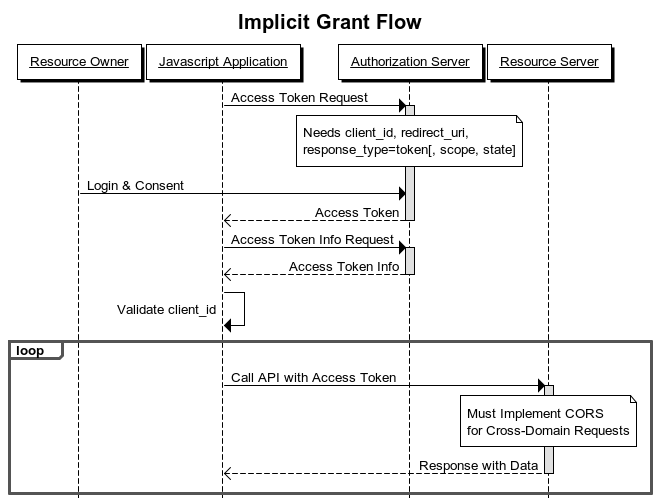
\includegraphics[width=0.7\textwidth]{ImplicitGF}}%
}%
\caption{Implicit Grant Flow.}
\label{fig:ImplicitGrantFlow}
\end{figure}

\item \textbf{Resource Owner Password Credentials Grant} (Figura \ref{fig:ResourceOwnerPasswordCredentialsFlow}). Se suele utilizar cuando el servidor de autorización y el cliente parten de la misma entidad, ya que las credenciales se mandan al cliente y éste a su vez las lanza al servidor de autorización. Bajo nuestro punto de vista aún cuando
haya completa confianza entre el cliente y el servidor de autorización sería mas serio utilizar \texttt{Authorization Code Grant}.

\begin{figure}[H]
\centering
{%
\setlength{\fboxsep}{0pt}%
\setlength{\fboxrule}{1pt}%
\fbox{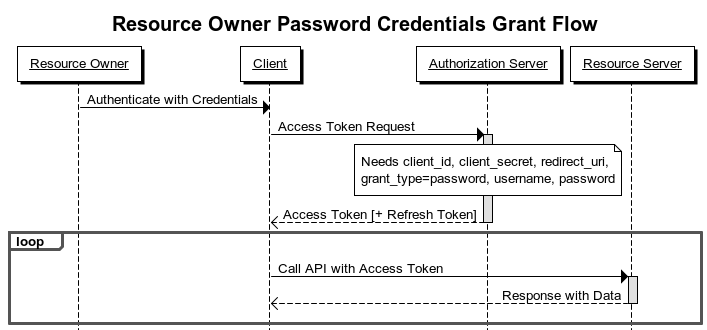
\includegraphics[width=0.7\textwidth]{ResourceOwnerPassCredGF}}%
}%
\caption{Resource Owner Password Credentials Grant Flow.}
\label{fig:ResourceOwnerPasswordCredentialsFlow}
\end{figure}

\item \textbf{Client Credentials Grant} (Figura \ref{fig:ClientCredentialsFlow}). Normalmente este tipo de autorización se usa cuando el cliente es a la vez el \texttt{Resource Owner}. En este caso no se requiere autentificación por parte del usuario.

\begin{figure}[H]
\centering
{%
\setlength{\fboxsep}{0pt}%
\setlength{\fboxrule}{1pt}%
\fbox{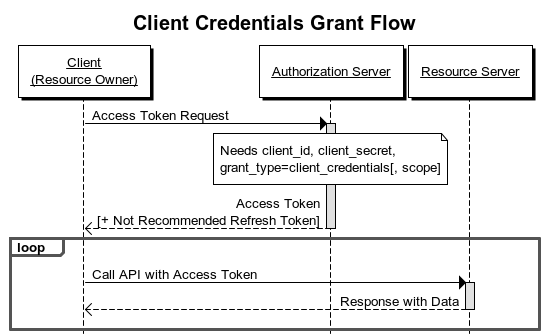
\includegraphics[width=0.7\textwidth]{ClientCredentialsGF}}%
}%
\caption{Client Credentials Grant Flow.}
\label{fig:ClientCredentialsFlow}
\end{figure}

\end{enumerate}
\noindent
En nuestro sistema utilizamos \textbf{Authorization Code Grant} ya que es el más seguro y a la vez es una manera de utilizar el caso de uso más común de este protocolo de seguridad, pues simplemente cambiando un par de líneas de código podríamos habilitar
la autenticación mediante Google, Facebook o cualquier otro sistema usado para la autenticación.\\

\subsection{Implementación de microservicios}
\vspace{2mm}
\noindent
Después de hablar de los aspectos de diseño y analizar la orquestación de nuestros microservicios, vamos a hablar de la implementación de los mismos, así como de las herramientas utilizadas.
Principalmente hemos usado JAVA, más concretamente el framework \textit{Spring} de ese lenguaje, dado el alto acoplamiento y la facilidad de implementación de la capa de Netflix OSS en ese framework. Para ver cómo hemos realizado
la implementación lo mejor es ver como hemos implementado alguno de estos microservicios, a su vez veremos pinceladas del funcionamiento de alguno de los componentes de nuestra capa de orquestación.

El hecho de utilizar \textit{Spring} viene motivado principalmente por ser considerado el framework de JAVA más utilizado a la hora de realizar desarrollo de \textit{back-end} en el \textit{Developer Survey} de Stackoverflow tanto en el año 2016 \cite{stackOverflowDev_2016} como en el 2017 \cite{stackOverflowDev_2017}.
Por lo que me motivó la idea de aprender una nueva tecnología que está muy bien considerada a la hora de realizar desarrollo web en JAVA. Además, este framework cuenta con una herramienta muy util llamada \textit{Spring Boot} \cite{spring_boot}, la cual
nos permite crear un proyecto arquetipo de manera rápida ya funcional, con todas las dependencias que consideremos oportunas, ahorrándonos posibles problemas con las versiones de las librerías que utilicemos. También proporciona un pequeño
servidor \textit{Tomcat} embebido lo cual hace que nuestro microservicio sea casi completamente independiente a la hora de ejecutarse.

Una vez ya comentado cómo se han creado cada uno de los microservicios, nos centraremos en una de ellos con más detenimiento, concretamente \textbf{Neo4jService}. Lo primero es ver el Scaffolding del mismo para tener una idea de como estructuramos nuestro microservicio en la Figura \ref{fig:ScaffoldingWhayaAPIneo}.

\begin{figure}[H]
\centering
{%
\setlength{\fboxsep}{0pt}%
\setlength{\fboxrule}{1pt}%
\fbox{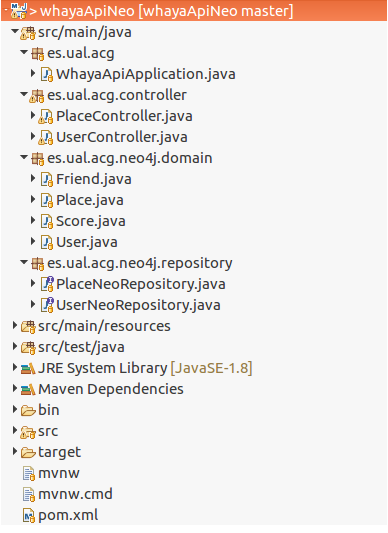
\includegraphics[width=0.4\textwidth]{whayaAPIFolders}}%
}%
\caption{Scaffolding WhayaAPIneo.}
\label{fig:ScaffoldingWhayaAPIneo}
\end{figure}
\noindent
Sobre la anterior figura vamos a dilucidar una serie de puntos para intentar explicar cada uno de los elementos que se pueden observar:

\begin{enumerate}[label=\alph*)]
\item En \textbf{src/main/java} encontraremos los archivos fuente de nuestra aplicación, donde observamos una serie de subcarpetas que tienen más que ver con la
separación de componentes de nuestra aplicación, a saber:
\begin{itemize}
\item \texttt{es.ual.acg} encontramos \texttt{WhayaApiApplication.java} que es basicamente el punto de entrada de nuestra aplicación
donde tenemos implementado también todo lo relacionado con la llamada al servicio de autenticación. En el código que mostramos a continuación (Listing \ref{lst:WhayaApiApplication})
podemos ver una serie de decoradores en clases y métodos que nos ayudan a definir ciertas propiedades de nuestra aplicación de \textit{Spring}.
Prestamos especial atención a algunos, como es el caso de \texttt{@EnableNeo4jRepositories} que nos dice que esta app va a usar elementos de \textit{Spring Data Neo4j}
como persistencia de datos. También la anotación \texttt{@EnableEurekaClient} que indica que este servidor de API pertenece a una infraestructura gobernada por \texttt{Eureka}. \texttt{@SpringBootApplication}
nos viene a decir que esta aplicación es una aplicación de \textit{Spring Boot} con un servidor web embebido. Más abajo, en \texttt{@EnableResourceServer} y \texttt{@EnableGlobalMethodSecurity}, indicamos
que estamos utilizando una configuración de seguridad global con un microservicio externo para la ejecución de la misma. 

\begin{minipage}{\linewidth}
\begin{lstlisting}[language=java,basicstyle=\ttfamily\scriptsize, caption={\texttt{WhayaApiApplication.java}.},captionpos=b, label={lst:WhayaApiApplication}]
package es.ual.acg;
import org.springframework.boot.SpringApplication; ...
@EnableTransactionManagement @ComponentScan
@EnableNeo4jRepositories @EnableEurekaClient
@SpringBootApplication
public class WhayaApiApplication {
    public static void main(String[] args) {
        SpringApplication.run(WhayaApiApplication.class, args);
    }
    @Primary @Bean
    public RemoteTokenServices tokenService() {
        RemoteTokenServices tokenService = new RemoteTokenServices();
        tokenService.setCheckTokenEndpointUrl(
            "http://zuul:8080/authservice/oauth/check_token");
        tokenService.setClientId("ClientIdPassword");
        tokenService.setClientSecret("secret");
        return tokenService;
    }
    @Configuration @EnableResourceServer
    @EnableGlobalMethodSecurity(prePostEnabled = true)
    public class OAuth2ResourceServerConfig 
        extends GlobalMethodSecurityConfiguration {
        @Override
        protected MethodSecurityExpressionHandler createExpressionHandler() {
            return new OAuth2MethodSecurityExpressionHandler();
        }
    }
}
\end{lstlisting}
\end{minipage}

\item \texttt{es.ual.acg.neo4j.domain} cuenta con archivos POJO (Plain Old Java Object) que definen los Nodos y relaciones de nuestra base de datos \textit{Neo4j}. Como ejemplo el siguiente fragmento de código (Listing \ref{lst:User}), donde
vamos a declarar ciertas propiedades de nuestro nodo User y decoramos las relaciones que si son complejas contarán con ciertas clases que representan propiedades de las relaciones, con sus \textit{getters} y \textit{setters}.
En la misma vemos cómo contamos con un índice declarado implicitamente \textbf{email}, este índice es muy importante en nuestro sistema ya que es el que da consistencia, y por el cual relacionamos todas las
distintas bases de datos que utilizamos en nuestro sistema.

\begin{minipage}{\linewidth}
\begin{lstlisting}[language=java,basicstyle=\ttfamily\scriptsize, caption={Ejemplo POJO \texttt{User.java}.},captionpos=b, label={lst:User}]
package es.ual.acg.neo4j.domain;

import java.util.ArrayList; ...
@NodeEntity
public class User {

    @GraphId private Long id;
    @Index(unique=true) private String email;
    private String name;
    private String avatar;
    private List<Friend> friend;
    private List<Score> score;
    private List<Place> places;
    
    public User() {
        score = new ArrayList<Score>();
        friend = new ArrayList<Friend>();
        this.places = new ArrayList<Place>();
    }
    ...
}
\end{lstlisting}
\end{minipage}
\item \texttt{es.ual.acg.neo4j.repository} en esta carpeta contamos con la ayuda de \textit{Spring Data}, vemos que el archivo ejemplo (Listing \ref{lst:PlaceNeoRepository})es una interfaz JAVA que hereda de \texttt{Graph\-Repository\textless Place\textgreater} lo cual por
defecto ya nos ofrece todas las operaciones CRUD sobre la entidad \texttt{Place}, y además, vemos que definimos una serie de métodos en esa interfaz, por lo que contamos con algo
más que las operaciones CRUD. Por un lado, el método \texttt{findByName(String name)}, es también parte de una serie de ayudas que nos ofrece \textit{Spring Data} para no tener
que implementar métodos simples. En este caso \texttt{findBy+nombre de propiedad} indica a \textit{Spring Data} que genere un código por debajo que tenga la funcionalidad de buscar un lugar en
este caso por su nombre. Por otro lado, vemos que tenemos dos métodos que tienen un decorador \texttt{@Query}, más concretamente los métodos \texttt{addToSpatialIndex()} y \texttt{closePlaces()},
esto indica a \textit{Spring Data} que genere unos métodos que cumplan con el comportamiento de la query que se indica. El primero de estos dos últimos métodos se encargan de introducir un lugar en el índice espacial
de nuestra base de datos y el otro de ofrecer los lugares que tenemos a cierta distancia.    

\begin{minipage}{\linewidth}
\begin{lstlisting}[language=java,basicstyle=\ttfamily\scriptsize, caption={Ejemplo repository \texttt{PlaceNeoRepository.java}.},captionpos=b,label={lst:PlaceNeoRepository}]          
package es.ual.acg.neo4j.repository;
import java.util.List; ..

@Component
public interface PlaceNeoRepository extends GraphRepository<Place> {

    @Query("MATCH (n:Place) WHERE NOT (n)<-[:RTREE_REFERENCE]-() AND n.name = {name} CALL spatial.addNode('LocationsLayer', n) YIELD node RETURN node")
    Place addToSpatialIndex(@Param(value = "name") String name);

    Place findByName(String name);
    
    
    @Query("CALL spatial.withinDistance('LocationsLayer',{longitude:{longitude},latitude:{latitude}},{distance})")
    List<Place> closePlaces(@Param(value = "latitude") double latitude, @Param(value = "longitude") double longitude, @Param(value = "distance") double distance);
}
\end{lstlisting}
\end{minipage}
\item \texttt{es.ual.acg.controller}. En esta carpeta tenemos controladores de usuario y lugares. En sí esto no es necesario si solo utilizamos las operaciones CRUD,
ya que las interfaces que heredan de los tipos \texttt{Repository} nos permitirian de manera automática mostrar estas operaciones si fuesen las únicas que necesitamos. En nuestro caso, contamos con comportamientos
un tanto especiales en alguno de los metodos, como por ejemplo puede ser el \textit{delete}, en el cual no borramos el nodo en concreto, sino que lo colocamos como no visible para seguir teniendo
consistencia en la base de datos. Por lo tanto, solo creamos controladores porque queremos ir un poco mas allá de lo que serían operaciones básicas, y para indicar que es un controlador, lo hacemos con
\texttt{@RestController}. En el ejemplo que se muestra en el siguiente código (Listing \ref{lst:userController}) comprobamos que utilizamos otros decoradores, como los decoradores de mapeo de rutas \texttt{@PostMapping...} para indicar
el tipo de petición y ruta al que corresponde cada método, \texttt{@lstinline\{@Autowired\}} que indica que automáticamente va a configurar que injectar, sin tener que realizar ninguna instanciación de nuestra parte, o
\texttt{@HystrixCommand} que indica el método que va a saltar cuando \textit{Hystrix} lo requiera.

\begin{minipage}{\linewidth}
\begin{lstlisting}[language=java,basicstyle=\ttfamily\scriptsize, caption={Ejemplo controlador \texttt{UserController.java}.},captionpos=b, label={lst:userController}]
    
package es.ual.acg.controller;
import java.util.ArrayList; ...


@RestController
@RequestMapping("/users")
public class UserController {

    @Autowired
    private UserNeoRepository userNeoRepository;

    @HystrixCommand(fallbackMethod = "defaultUser")
    @PostMapping("")
    public ResponseEntity createUser(@Param(value = "email") String email, @Param(value = "name") String name, @Param(value = "avatar") String avatar) {

        try {
            User aux = new User(email, name, avatar);
            User compareAux = this.userNeoRepository.findByEmail(email);
            if (compareAux != null) {
                return new ResponseEntity("User already created", HttpStatus.CONFLICT);
            }
            userNeoRepository.save(aux);
            return new ResponseEntity(aux, HttpStatus.OK);
        } catch (Exception e) {
            return new ResponseEntity(e, HttpStatus.INTERNAL_SERVER_ERROR);
        }

    }
    public ResponseEntity defaultUser(@Param(value = "email") String email, @Param(value = "name") String name) {
        return new ResponseEntity(null, HttpStatus.BAD_GATEWAY);
    }
}
\end{lstlisting}
\end{minipage}

\end{itemize}
\item En la carpeta \textbf{resources} introducimos archivos con los parámetros de configuración global de nuestro microservicio, cosas como datos de conexión a \textit{Neo4j} o \textit{Rabbitmq}, apuntamos la
dirección de \textit{Eureka}, etc. En el siguiente código (Listing \ref{lst:applicationProperties}) se puede ver un ejemplo sencillo.
\begin{minipage}{\linewidth}
\begin{lstlisting}[basicstyle=\ttfamily\scriptsize, caption={Ejemplo \texttt{application.properties}.},captionpos=b, label={lst:applicationProperties}]    
spring.application.name=neoservice
server.port=0

spring.data.neo4j.uri=bolt://neo4j:7687
spring.data.neo4j.username=neo4j
spring.data.neo4j.password=passP

eureka.client.serviceUrl.defaultZone: ${EUREKA_URI:http://zuul:8080/eureka/eureka}
eureka.instance.instance-id=${spring.application.name}:${random.int}
eureka.instance.preferIpAddress=true

spring.rabbitmq.host=rabbitmq
spring.rabbitmq.port=5672
spring.rabbitmq.username=guest
spring.rabbitmq.password=guest   
\end{lstlisting}
\end{minipage}
\end{enumerate}

\noindent
A parte de este tipo de microservicios contamos con los de la capa de orquestación, los cuales prácticamente \textit{Spring Boot} nos los da ya implementados.
Simplemente seleccionando el arquetipo oportuno y cambiando opciones de configuración tendremos levantada la capa de orquestación. Por poner un ejemplo,
una vez creamos el arquetipo \textit{Eureka Server} de \textit{Spring Boot}, literalmente tendremos ya levantado el servidor de \textit{Eureka}, solo teniendo que configurar el archivo \texttt{application.properties} del mismo con la configuración del puerto donde queremos levantarlo.
Para ver lo simple que es, en el siguiente código (Listing \ref{lst:EurekaApplication}) tenemos la implementación de nuestro servidor de \textit{Eureka}.

\begin{lstlisting}[language=java,basicstyle=\ttfamily\scriptsize, caption={\texttt{EurekaApplication.java}.},captionpos=b,label={lst:EurekaApplication}]
            
package es.ual.acg;

import org.springframework.boot.SpringApplication;
import org.springframework.boot.autoconfigure.SpringBootApplication;
import org.springframework.cloud.client.discovery.EnableDiscoveryClient;
import org.springframework.cloud.netflix.eureka.server.EnableEurekaServer;

@SpringBootApplication
@EnableEurekaServer
@EnableDiscoveryClient
public class EurekaApplication {

    public static void main(String[] args) {
        SpringApplication.run(EurekaApplication.class, args);
    }
}
\end{lstlisting}
\noindent
Por último, contamos con un servicio en particular que es el que trata con datos en tiempo real, mediante el framework de \textbf{Socket.io}, implementado en \texttt{Node.js}. El framework nos permite enviar mensajes sobre el protocolo
WebSocket y básicamente trata de responder a ciertos mensajes con otros. Para intentar entenderlo mejor vamos a ver un fragmento del código (Listing \ref{lst:ws}) de nuestro microservicio.

\begin{lstlisting}[language=JavaScript,basicstyle=\ttfamily\scriptsize, caption={Ejemplo socket.io \texttt{app.js}.},captionpos=b, label={lst:ws}]
            
var express = require('express');
var app = express();
app.set('port', process.env.PORT || 9000);
var request = require('request');
var server = require('http').Server(app);
var io = require('socket.io')(server);
var port = app.get('port');

app.use(express.static('public'));

server.listen(port, function () {
    console.log("Server listening on: http://localhost:%s", port);
});

function User(email, name, socketId) {
    this.email = email;
    this.name = name;
    this.socketId = socketId;
}
var users = [];

io.sockets.on('connection', function (socket) {

    socket.on('connected', function (data) {


        socket.user = new User(data.email, data.name, socket.id);
        users.push(socket.user);
        console.log('users:' + JSON.stringify(users))

    });

    socket.on('addConnectionFriend', function (data) {

        for (var i = 0; i < users.length; i++) {

            if (data.friend == users[i].email) {
                socket.to(users[i].socketId).emit("userConnected", { 'email': socket.user.email, 'name': socket.user.name, 'socketId': socket.id });
                socket.emit("userConnected", { 'email': users[i].email, 'name': users[i].name, 'socketId': users[i].socketId });
            }
        }
    });
});
\end{lstlisting}
\newpage
\noindent
En los métodos mostrados de este servicio vemos lo que hacemos cuando nos conectamos al mismo. Simplemente nos incluimos en una variable global del servidor donde estan todos los usuarios conectados.
A continuación con el mensaje \textit{addConnectionFriend} comprobamos si el usuario amigo al que queremos decirle que estamos conectados está en la lista de usuarios conectados, y de ser así mandaremos un mensaje
a ese usuario con nuestro \texttt{socketId} y a la vez recuperamos para nosotros el \texttt{socketId} del usuario. En ese momento tendremos la posibilidad de comunicarnos de manera directa entre ambos.
Este servicio queda fuera de la capa de orquestación, dado que no permite réplica, ya que existe la problemática de que si tenemos varias réplicas esa lista de usuarios global cabría la posibilidad de que estuviese particionada
provocando que se diese el caso de que dos usuarios estuviesen conectados sin que sean visibles entre sí. Esta problemática puede tener distintas soluciones pero se sale del contexto de este proyecto. 
Este servicio es el que se encarga de llevar todo lo relacionado con cuando se conectan tus amigos al sistema, el chat y por ejemplo el que pasa tu posición a tus amigos. Al realizar este microservicio es interesante ver como
hemos realizado la conexión y la comunicación de datos 1 a 1 para aumentar la privacidad del sistema. El siguiente diagrama de secuencia (Figura \ref{fig:connectionToWs}) ilustra el funcionamiento del código anterior.

\begin{figure}[H]
\centering
{%
\setlength{\fboxsep}{0pt}%
\setlength{\fboxrule}{1pt}%
\fbox{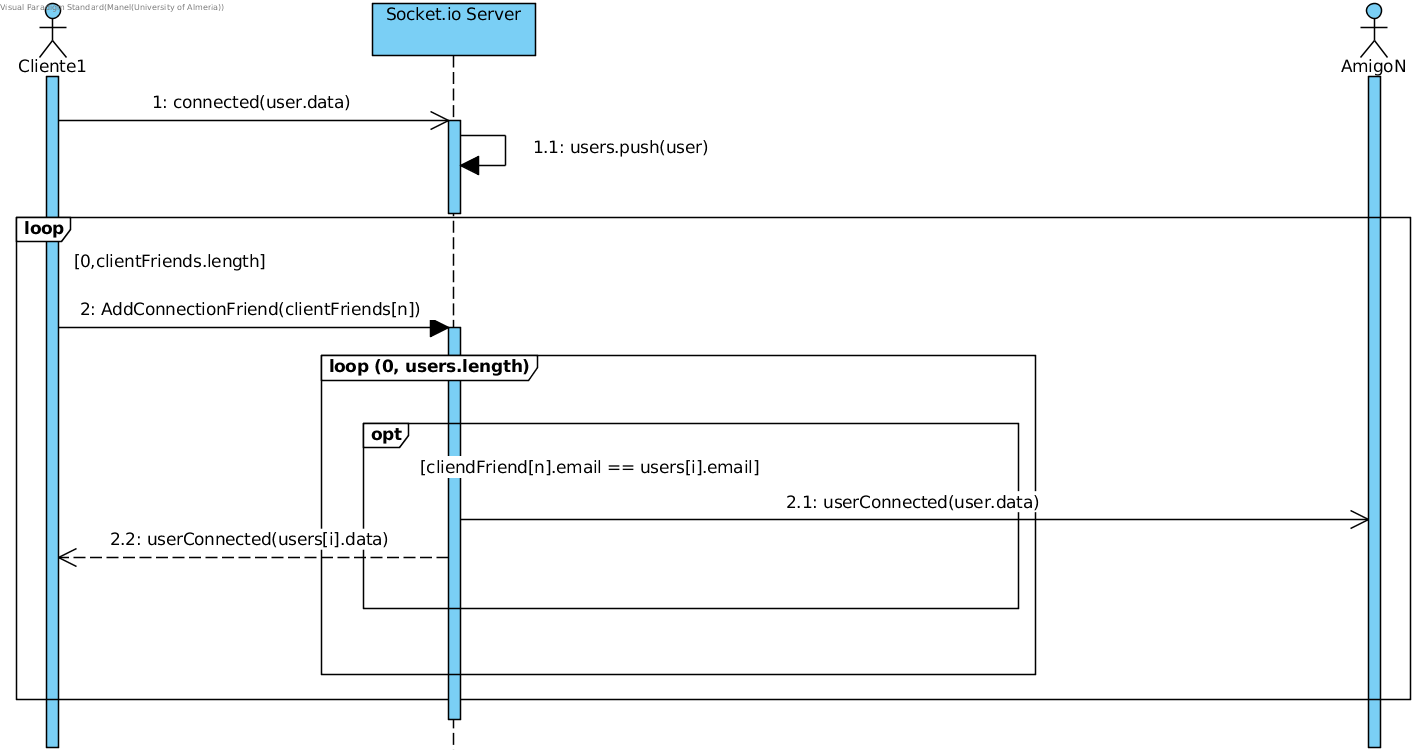
\includegraphics[width=1\textwidth]{connectionToWs}}%
}%
\caption{Diagrama de secuencia WS.}
\label{fig:connectionToWs}
\end{figure}
